\documentclass[UTF8]{ctexart}
\usepackage{xcolor}
\usepackage{enumerate}
\usepackage{graphicx}
\usepackage{geometry}
\geometry{left = 2.5cm,right= 2cm}
\title{Logistic Regression - Detailed overview}
\author{DuLi}
\date{\today}
\begin{document}
\maketitle
\newpage

\begin{center}
\includegraphics[width = 6in]{Logistic.png}
\end{center}

\section{逻辑回归}
\subsection{逻辑回归概览}
逻辑回归最早在二十世纪早期被用于生物学领域,之后在社会科学领域有所使用。
逻辑回归常被用作分类问题。
例如:
\begin{enumerate}[*]

\item 来预测垃圾邮件。

\item 预测肿瘤是否是良性的。

\end{enumerate}

试想如下情景,我们准备将一封邮件归类为垃圾邮件或者不是。如果使用线性回归来解决这个问题,就需要设定一个阈值。如果事实上是一个恶性类,我们计算出来的值是0.4,但是阈值是0.5,纳闷就会被分类为良性,这就会造成比较严重的问题。
从这我们可以看出,线性回归不太适合做分类问题,线性回归是不受限制的,这就引出了逻辑回归,将值严格的控制在0和1之间。

\subsection{Simple Logictic Regression}
\label{sub:simple_logictic_regression}

$$Output = 0 or 1$$
$$Hypothesis => Z = WX+B$$
$$h(x) = sigmoid(Z)$$

\subsection{Sigmoid Function
} (fold)
\label{sub:sigmoid_function_}

\begin{center}
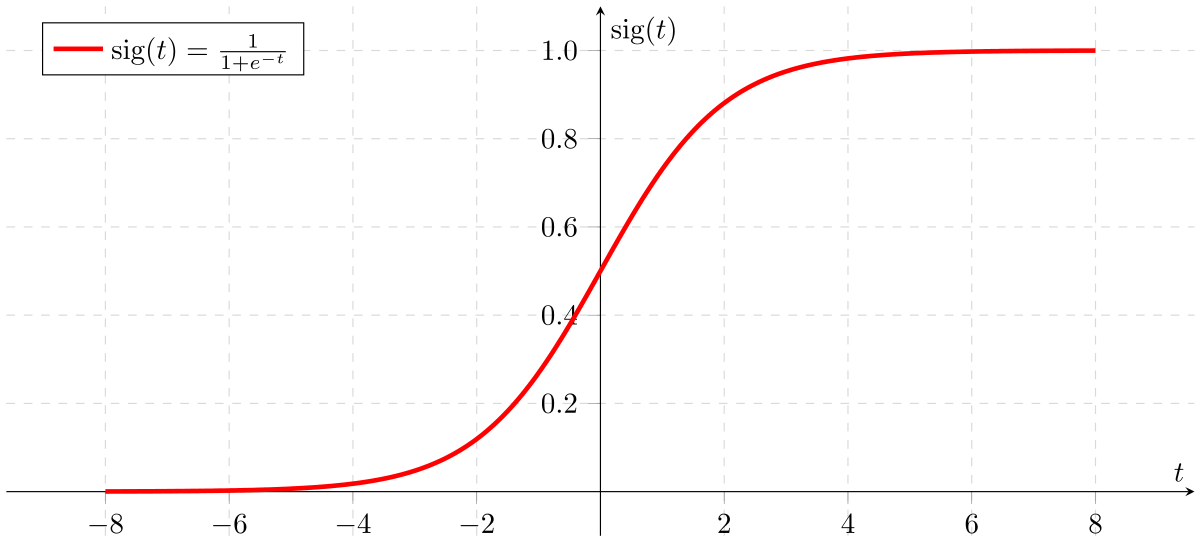
\includegraphics[width = 6in]{sigmoid.png}
\end{center}

sigmoid函数的一大特征在于,当X趋于正无穷时,函数值为1,当趋近于负无穷时,函数值为0.

\subsection{Analysis of the hypothesis} % (fold)
\label{sub:analysis_of_the_hypothesis}

基于这个假设的输出是估计概率。这用来表示当给定一个X时,对于预测的值有多大的置信度。

\begin{center}
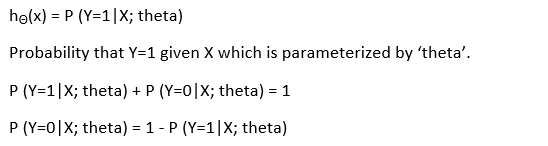
\includegraphics[width = 6in]{representation.png}
\end{center}

\end{document}